% Asset ID: AS1TrigonometricRatiosTIKZ-006
% Source: P1-Chp9 pp.20-21
% Related section: Area Formula
% Purpose: Included angle for area formula
\documentclass[tikz,border=8pt]{standalone}
\usepackage{amsmath}
\usetikzlibrary{angles,quotes,calc,arrows.meta}
\begin{document}
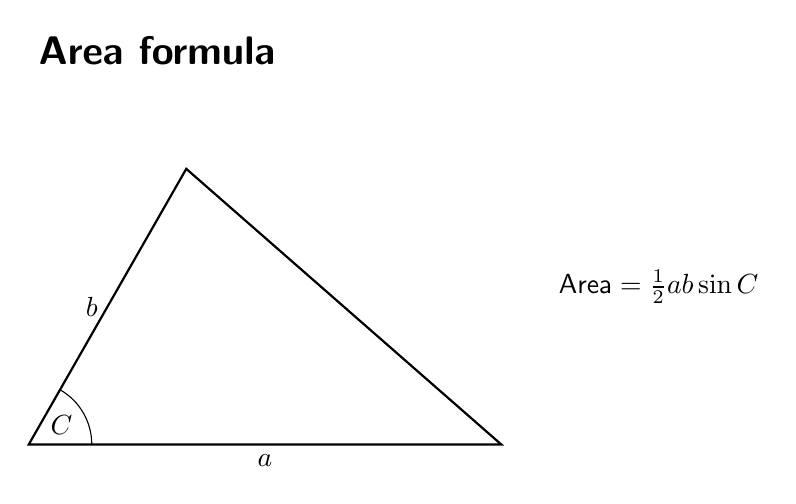
\begin{tikzpicture}[scale=1.0, every node/.style={font=\sffamily}]
\node[font=\sffamily\bfseries\Large, anchor=west] at (0,5) {Area formula};
\coordinate (C) at (0,0);\coordinate (A) at (6,0);\coordinate (B) at (2,3.5);\draw[thick] (C)--(A)--(B)--cycle;\pic[draw,"$C$",angle radius=.8cm] {angle=A--C--B};\node[below] at ($(C)!0.5!(A)$) {$a$};\node[left] at ($(C)!0.5!(B)$) {$b$};\node at (8,2) {$\text{Area}=\frac12ab\sin C$};
\end{tikzpicture}
\end{document}
